\usepackage[top=1.5cm,bottom=3cm,inner=1.8cm,outer=2cm]{geometry}
%\geometry{showframe}
%\usepackage[all]{nowidow}
\usepackage{makeidx}

\usepackage{titlesec}

%Titlepage
\usepackage{titling}
%\pretitle{
% \vspace{4cm}
% \begin{center}
% \Huge
%}
\providecommand{\subtitle}[1]{%
  \posttitle{%
    \par\large#1\normalsize\linebreak
    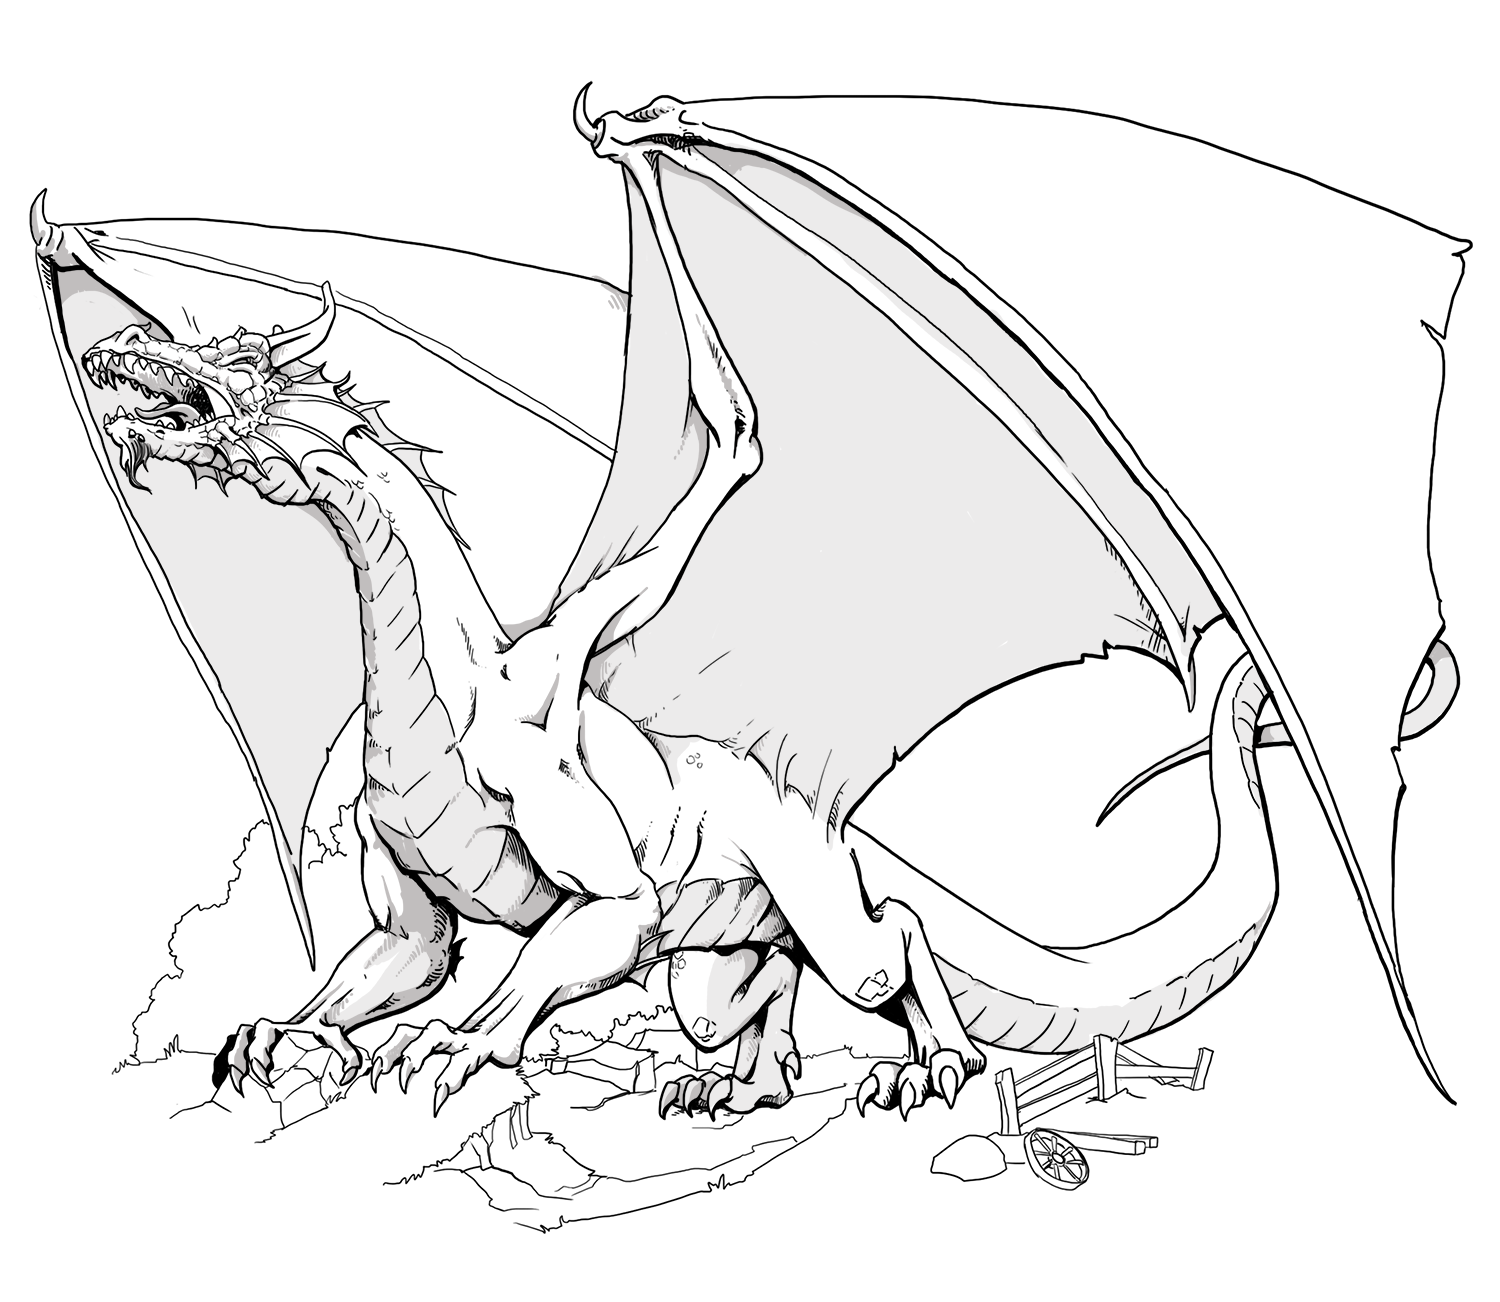
\includegraphics[width=0.8\textwidth]{img/DnD_Dragon.png}
	\linebreak
    
\includegraphics[width=1.8cm]{img/OSR-logo2.png}
    \end{center}
%  \newgeometry{bottom=3cm}
    }
}


%\renewcommand{\maketitle}{
% \begin{center}
% {\Huge\thetitle}\linebreak
% \providecommand{\subtitle}[1]{
%  \par\large#1\normalsize\linebreak
% }
% \end{center}
%} 

\titleformat{name=\section,page=odd}
  {\vfill\pagebreak\flushright\Large\scshape}
  {}
  {0em}
  {}

\titleformat{name=\section,page=even}
  {\vfill\pagebreak\flushleft\Large\scshape}
  {}
  {0em}
  {}

\titleformat{\subsection}
  {\vspace{.5cm}\center\scshape}
  {}
  {0em}
  {}

\titleformat{\subsubsection}
  {\center\itshape}
  {}
  {0em}
  {}[\titlerule]

\titleformat{\subsubsubsection}
  {\center\itshape}
  {}
  {0em}
  {}[\titlerule]

% Fonts
\usepackage[osf]{coelacanth}
%\usepackage{palatino}
\usepackage[T1]{fontenc}
%\input MorrisIn.fd

\usepackage{lettrine}
%\usepackage{Zallman}
%\renewcommand{\LettrineFontHook}{\Zallmanfamily}
\setcounter{DefaultLines}{3}

\usepackage{fancyhdr}
\pagestyle{fancy}
\renewcommand\headrulewidth{0pt} % no line between document and header
\fancyhead{} % clear header
\fancyfoot{} % clear footer
\fancyfoot[LE,RO]{\thepage} % page at left on even and right on odd pages

% make quote boxes:
\usepackage{framed,color}
\definecolor{shadecolor}{rgb}{1,0.8,0.3}
%\renewenvironment{quote}{\begin{framed}}{\end{framed}}

%\usepackage{multicol}
\usepackage[many]{tcolorbox}% version 2.80 (2014/03/31)
\usepackage[section]{placeins}
%\NewTColorBox{character}{ s O{!htbp} }{%
%  floatplacement={#2},
%  IfBooleanTF={#1}{float*,width=\textwidth}{float},
%  colframe=blue!50!black,colback=blue!10!white,% any tcolorbox
%  }
%\newenvironment{character}{\begin{shaded}}{\end{shaded}}
\newenvironment{character}{\begin{tcolorbox}}{\end{tcolorbox}}

\makeindex
